\chapter{Experimental Setup}

\section{Data}

Training and testing data for the experiment comes from the \textsc{Delphes} and \textsc{Geant4} simulators. These datasets include information about the detector response to collision events as well as information about the geometry of the ATLAS detector. During collision events, particles may pass through several elements of the detector and register multiple hits. These hits are combined in a processing step to output information about the reconstructed particles. Within each event, up to 200 particles are reconstructed to form constituents to the event. Samples contain four-vectors for the jet and four-vectors for each constituent within the jet. For each event, the jet four-vector contains the invariant mass $m$, transverse momentum $p_T$, $\eta$, and $\phi$ features. For each reconstructed particle, we record the Energy $E$, $p_T$, $\eta$, and $\phi$ as a constituent four-vector. All angles have units of radians, energy values are in units of TeV, and momentum are in units of TeV/c where c is the speed of light in m/s.

Each dataset is split into 16 million sample training sets and 5 million sample validation sets. Approximately half of each dataset is signal and the other half is background. Because each sample is generated independently and according to the same simulation process, they are assumed to be independently and identically distributed (IID). Samples are randomly shuffled before training. All base models are pretrained on all 16 million \textsc{Delphes} samples, while 2, 4, 8, or 16 million \textsc{Geant4} samples are used for target model training.

Although both datasets model the same interactions, the differences in simulation method output slightly different data distributions as shown in Figure \ref{fig:feature_hists}. Most notably, the two simulation datasets have different centers for the azimuthal coordinate $\phi$, though this can easily be corrected with a recentering procedure. The \textsc{Geant4} simulation also produces samples with higher variance in $\eta$. These differences in distribution pose a challenge for the transfer learning process as the model will need to relearn relevant features under a new regime. In general, the more similar the pretraining and fine-tuning data sets are, the easier it will be for a model to adapt to the data distribution shift when transferring parameters.

\begin{figure}
    \centering
    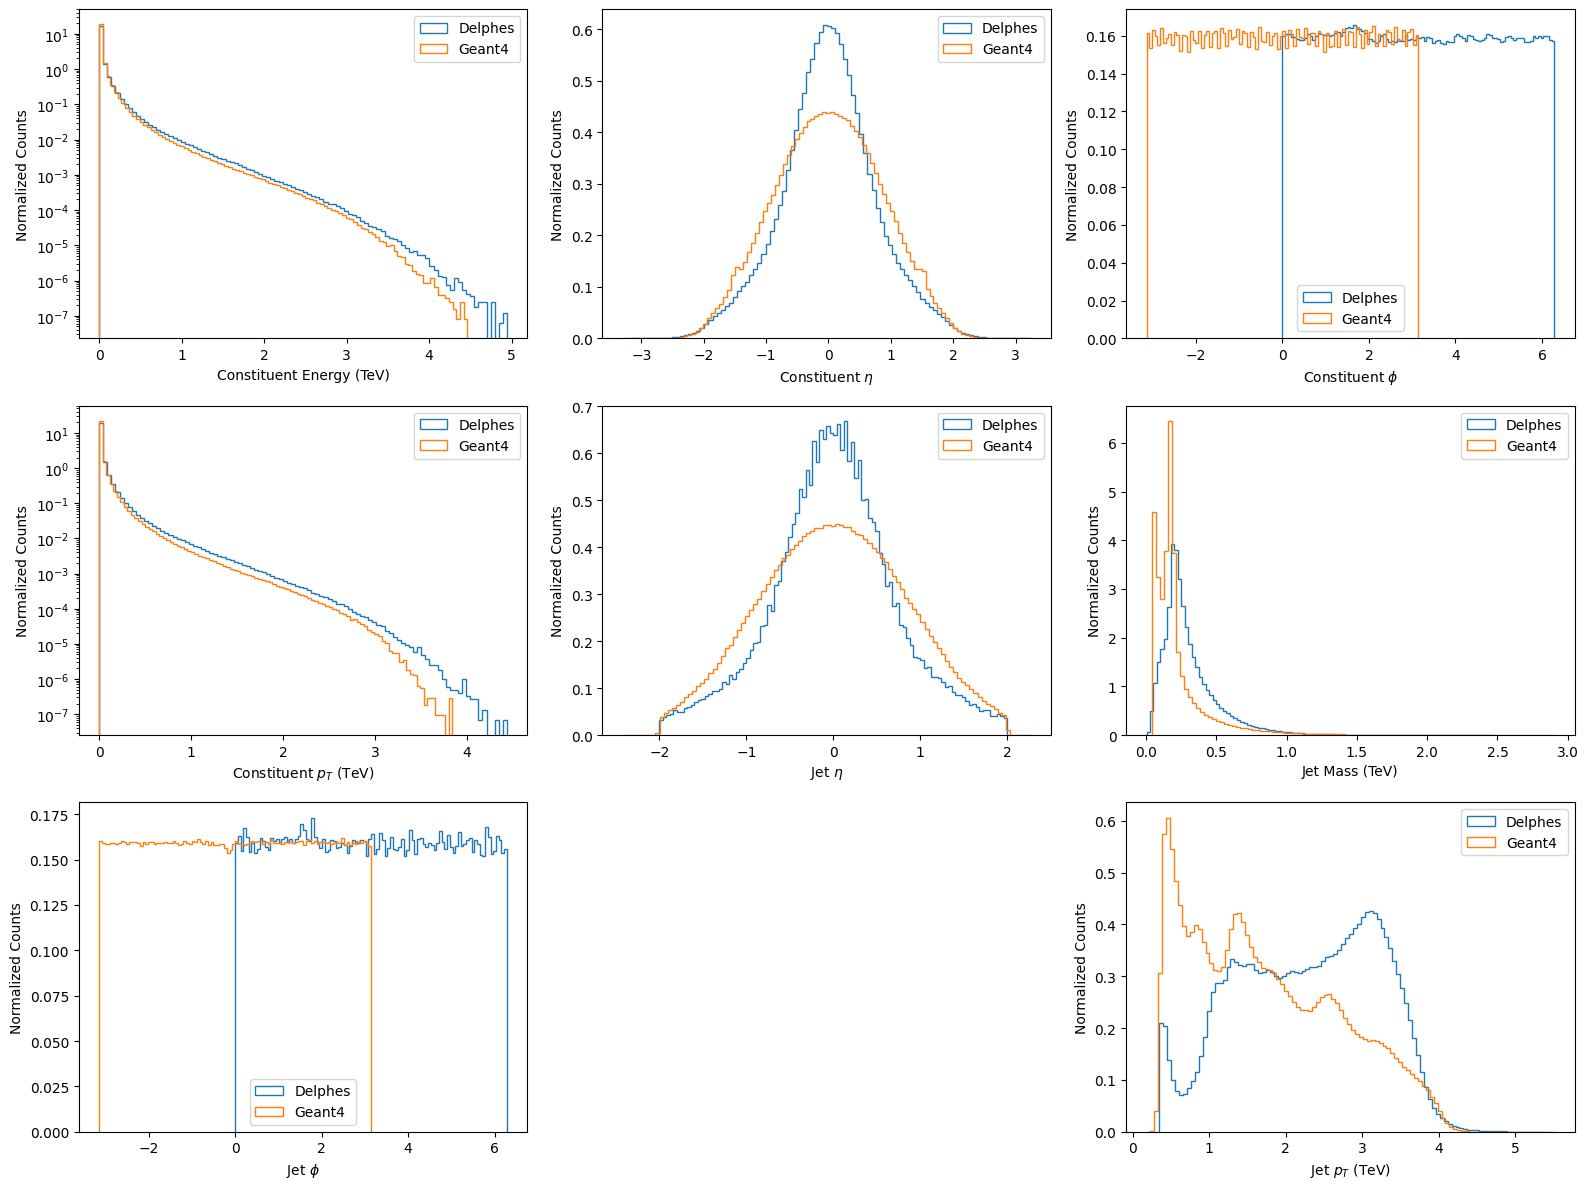
\includegraphics[width=1\linewidth]{figures/feature_hists.png}
    \caption{Distributions of features before preprocessing. Zero-padded constituents are not included in plots.}
    \label{fig:feature_hists}
\end{figure}

The four-vectors for jet-level features are always populated with values. However, simulations for constituent-level four-vectors set an upper bound on the number of constituents recorded to 200. Constituent data is stored in four fixed-size arrays of size ($N$ x 200) where $N$ is the number of samples. In the case of an event containing fewer than 200 constituents, unused constituent slots are zeroed out. Otherwise, the top 200 constituents sorted by largest $p_T$ are kept. The constituent feature distributions shown in figure \ref{fig:feature_hists} only count non-zero constituents. Due to the differences in simulation fidelity, there is also a difference in the sparsity of constituent data, or the proportion of constituents that are unfilled. \textsc{Delphes}, the lower fidelity simulation method, has $33.254\%$ of constituents filled with values while \textsc{Geant4} has just $27.939\%$. \textsc{Delphes} simulations produce more constituents due to the smearing method used during simulation. This difference in data distribution is clearly seen in Figure \ref{fig:num_constituents_hist}.

\begin{figure}
    \centering
    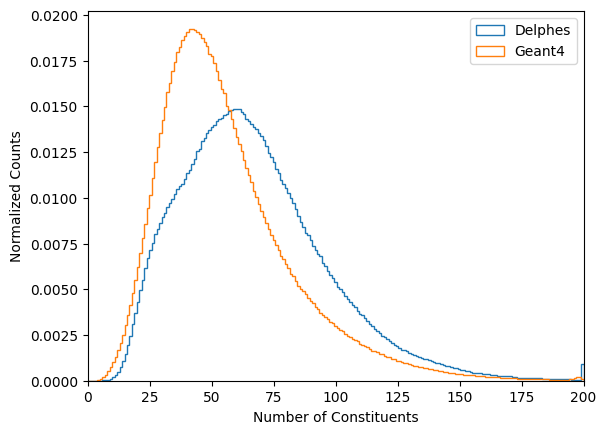
\includegraphics[width=0.5\linewidth]{figures/num_constituents_hist.png}
    \caption{Histogram of the number of nonzero constituents per sample.}
    \label{fig:num_constituents_hist}
\end{figure}

\subsection{Data Pre-Processing}
A common method in machine learning is to apply transformations to the features that will be helpful for the model to make more accurate predictions. These transformations can include functional applications to certain features or combinations of two or more features. Pre-processing can change the dimensionality of input data and thus increase model complexity and expressivity.

Datasets from both the \textsc{Delphes} and \textsc{Geant4} simulators are pre-processed in the same way according to the methods of Ref. \cite{ATL-PHYS-PUB-2022-039} using the accompanying Python script. The pre-processing transforms the constituent data by making use of symmetries in the detector geometry. First the $\eta$ and $\phi$ coordinates are centered by placing the constituent with highest $p_T$ value at the origin and the second-highest on the negative $\phi$ axis. If the third-highest $p_T$ constituent is on the negative $\eta$ half plane, then the coordinates are rotated about the $\phi$ axis. Both the energy $E$ and transverse momentum $p_T$ are replaced by their natural logarithms $\log E/\si{TeV}$ and $\log p_T c/\si{TeV}$ respectively.

Three additional features are also created and are defined as follows:

\begin{equation}
    \Delta R = \sqrt{\Delta\eta^2 + \Delta\phi^2}
\end{equation}

is the distance between a constituent and the jet axis in the pseudorapidity-azimuthal angle space,

\begin{equation}
    E_{norm} = log \left( \frac{E}{\sum\limits_{jet} E} \right)
\end{equation}

is the log-normalized energy, and

\begin{equation}
    p_{T,norm} = log \left( \frac{p_T}{\sum\limits_{jet} p_T} \right)
\end{equation}

is the log-normalized transverse momentum defined similarly to its energy counterpart.

These transformations were chosen from Ref. \cite{ATL-PHYS-PUB-2022-039} as they were shown to increase performance for top-tagging classifiers using similar model architectures. The distributions of these seven transformed constituent variables can be seen in Figure \ref{fig:preprocessed_hists}.

\begin{figure}
    \centering
    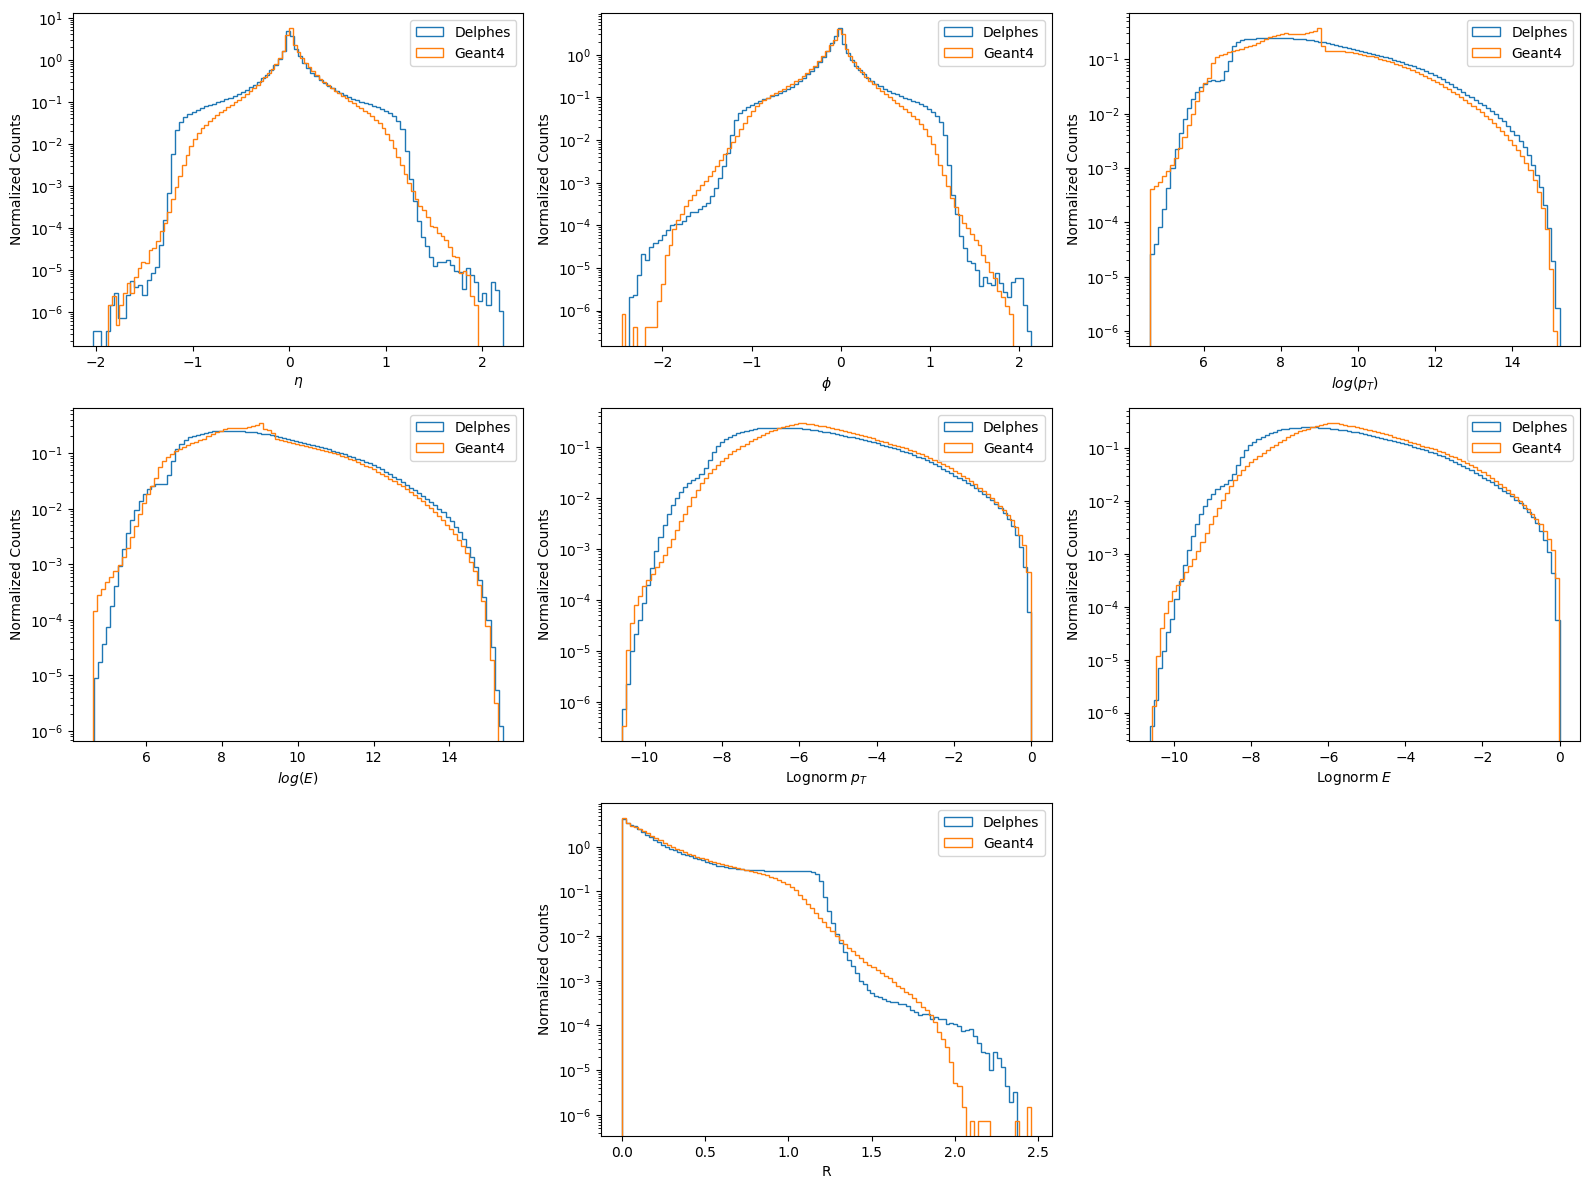
\includegraphics[width=1\linewidth]{figures/preprocessed_hists.png}
    \caption{Distributions of pre-processed feature variables. Zero-padded constituents are not included in plots.}
    \label{fig:preprocessed_hists}
\end{figure}

\section{Model}

A standard multi-layer perceptron (MLP) neural network is chosen as a representative and relatively simple model. The input layer contains all constituent-level pre-processed features for all 200 constituents. The input data is flattened into a single vector per sample.

A MLP with five hidden layers containing 400 nodes each is used. The binary cross entropy (BCE) loss, or log loss, is used as the loss function and given in Equation \ref{eq:bce_loss}. The MLP output layer is a single scalar node representing the predicted probability $\hat{y}$ that a given sample is a signal boosted top-quark decay event. A complete list of hyperparameters is given in Table \ref{tab:hyperparams} and were selected based on validation AUC in a hyperparameter search.

\begin{equation}
    L = y log\left(\hat{y}\right) + (1-y) log\left(1 - \hat{y} \right)
    \label{eq:bce_loss}
\end{equation}

\begin{table}[]
\centering
    \begin{tabular}{c|c}
    \hhline{==}
    \# Samples & No Pretrain \\ \hline
    Hidden Layers & 5 \\
    Nodes per hidden layer & 400 \\
    Activation Function & ReLU \\
    Optimizer & Adam \cite{kingma2017adam} \\
    Learning Rate & $10^{-4}$ \\
    Batch Size & 1024 \\
    \hhline{==}
    \end{tabular}
    \caption{MLP hyperparameters used for the final models.}
    \label{tab:hyperparams}
\end{table}

\section{Implementation}

Implementation of data loading, pre-processing, model training, and visualization are all done in \textsc{Python}. Neural network implementation and training used \textsc{JAX} \cite{jax2018github} and its supporting libraries \cite{deepmind2020jax}, including the \textsc{Flax} \cite{flax2020github} neural network library. Data for both \textsc{Delphes} and \textsc{Geant4} are stored in the \textsc{HDF5} file format which has optimizations for fast I/O. Experimental tracking and management was done with the Weights and Biases \cite{wandb} platform using the \textsc{wandb} Python library. Training runs were scheduled through the SLURM \cite{10.1007/10968987_3} workload manager on the NERSC Perlmutter compute cluster and used dedicated GPU nodes containing 4 NVIDIA A100 GPUs each \cite{perlmutter}. Test set inference was done on shared nodes. This setup allowed for parallelization of experiment runs which greatly increased research speed.

Five different values were used as random number generator (RNG) seeds to reduce variance in results. A base model was trained for each seed. Each variation of target model was trained five times using each base model for a total of $4 \times 2 \times 5 = 40$ (\# \textsc{Geant4} samples $\times$ pretraining $\times$ seeds) final target models.
